\documentclass[12pt, letterpaper]{article}
\usepackage[utf8]{inputenc}

\title{Control of robotic arm and gripper}
\author{Cristian Enrico Capalbo}
\date{\today}
\usepackage{graphicx}
\graphicspath{ {images/} }

\begin{document}

\maketitle

In the original design of the robot, the degrees of freedom of the arm and the gripper (the end effector) are controlled by means of a remote controller. 

\begin{figure}[h]
    \centering
    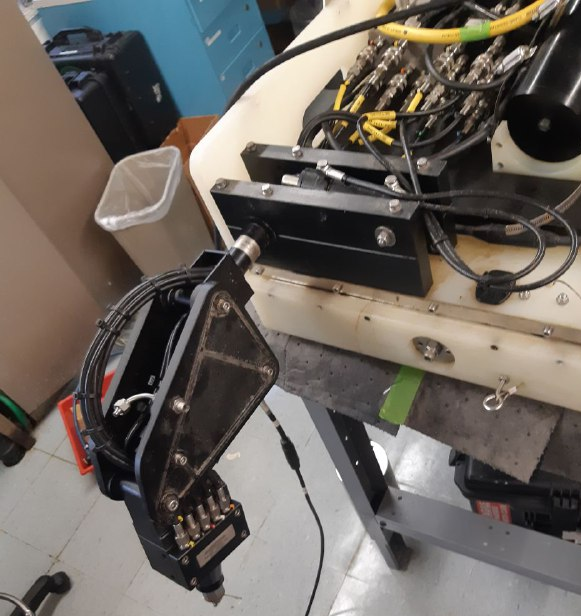
\includegraphics[width=0.25\textwidth]{arm}
    \caption{Robotic arm}
    \label{fig:arm}
\end{figure}

\begin{figure}[h]
    \centering
    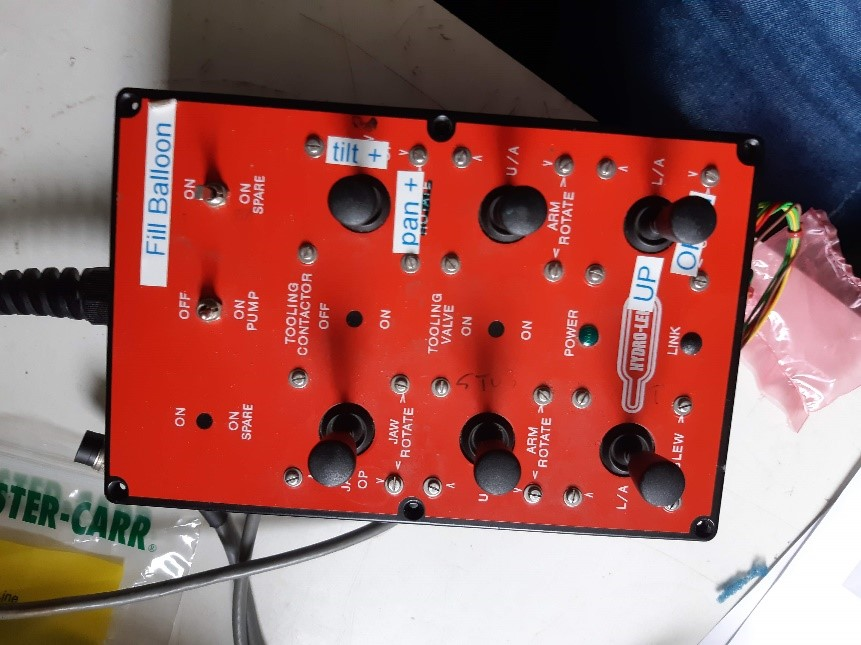
\includegraphics[width=0.25\textwidth]{remote.jpg}
    \caption{Remote controller}
    \label{fig:remote}
\end{figure}

\end{document}